\begin{figure}[t]

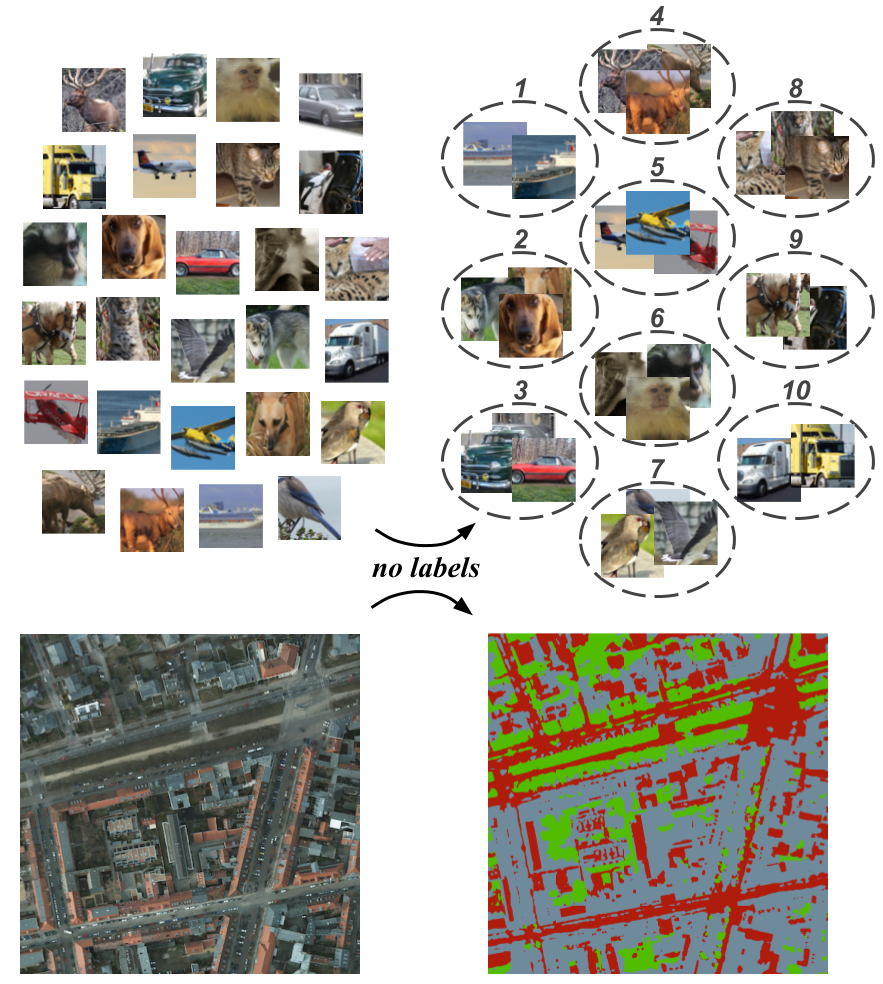
\includegraphics[height=1.1\textwidth]{experiments2_files/splash2.png}

\caption{\label{f:splash} Models trained with \methodnameshort on entirely unlabelled data learn to cluster images (top, STL10) and patches (bottom, Potsdam-3). The raw clusters found directly correspond to semantic classes (dogs, cats, trucks, roads, vegetation etc.) with state-of-the-art accuracy.  Training is end-to-end and randomly initialised, with no heuristics used at any stage.}
\end{figure}
